\documentclass[10pt, a4paper]{article}
\usepackage[T2A]{fontenc}
\usepackage[english, russian]{babel}

\usepackage{graphicx}
\graphicspath{{./figs/}}

\usepackage{amsmath}
\usepackage{amssymb}
\usepackage{mathtools}
\usepackage{physics}
\usepackage{upgreek}
\usepackage{sectsty}
\usepackage{color,soul}
\usepackage[colorlinks=true,allcolors=blue]{hyperref}
\sectionfont{\centering}

\usepackage{geometry}
 \geometry{
 a4paper,
 margin=25mm,
 }

\title{Билеты к кандидатскому экзамену по физике плазмы}
\date{}

\begin{document}

\newpage
\section{Термодинамика плазмы}
\label{sec.1}

\subsection{Понятие плазмы, квазинейтральность, микрополя, дебаевский радиус, идеальная и неидеальная плазма.}
\label{sec.1.1}

Плазма~\cite{kotelnikov}. Ссылка на уравнение~\eqref{eq.Euler}, Рис.~\ref{fig.1.2.1}.

У плазмы вводят т.н. параметр неидеальности, который есть $g = \frac{1}{n * r_d^3}$(Kroll, eq. 1.3.1). Когда 
$g \ll 1$ говорят, что плазма идеальна, т.к. в этом случае её свойства, как газа, схожи с идеальным газом.





~\cite{kotelnikov}. Ссылка на уравнение~\eqref{eq.Euler}, Рис.~\ref{fig.1.2.1}.


\begin{equation}
    \label{eq.Euler}
    e^{i \pi} + 1 = 0
\end{equation}

\subsection{Условие термодинамического равновесия, термическая ионизация, формула Саха, корональное равновесие, снижение потенциала ионизации.}
\label{sec.1.2}

Картинка

\begin{figure}[h!]
    \center{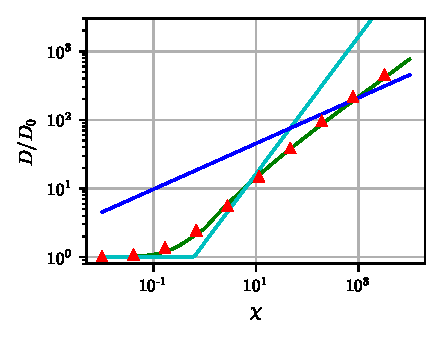
\includegraphics[width=85mm]{test.pdf}}
    \caption{\label{fig.1.2.1} Подпись.}
\end{figure}

\subsection{Вырождение плазмы, статистика Больцмана и Ферми—Дирака, модель Томаса—Ферми.}


\section{Элементарные процессы}
\label{sec.2}

\subsection{Столкновения заряженных частиц, дальнодействие.}
\label{sec.2.1}

[Ю.П. Райзер, Физика Газового разряда, 3-е изд, стр. 29]

Из всех сил взаимодействия между атомными частицами медленнее вceгo спадают с расстоянием (как $1/r^{2}$)  кулоновские силы. Они обладают наибольшим дальнодействием.
За время пролёта t мимо иона, электрон отклоняется на угол $\theta$ . Его можно оценить как отношение полученной поперечной скорости к изначальной скорости:

Основную роль в рассеянии играют столкновения с большим прицельным параметром $\rho$ (рассеяние на малые углы),реализуются при  $\rho > r_{0}$- Кулоновского радиуса (радиус при котором кин. энергия электрона равна потенциальной $ mv^{2}/2 = e^{2}/ r_{0} $,$ r_{0}=e^{2}/mv^{2} $). С другой стороны, потенциал иона спадает $\sim exp(-r/d)/r $. То есть основной вклад вносят столкновения с прицельным параметром от  $r_{0}$   до $d$ (радиус дебая).
Поэтому полное сечение для кулоновских рассеяний $\sigma= \pi*r_{0}^{2} \int_{r_{0}}^{d} r_{0} d\rho/\rho =\pi*r_{0}^{2}*ln{d/r_{0}}$

$ln{d/r_{0}}$ - Кулоновский логарифм.

Столкновения атомных частиц могут иметь упругий и неупругий характер. При упругом соударении меняются направления движения партнеров, происходит обмен импульсом и кинетической энергией, но внутренние энергии и состояния частиц остаются неизменными.

\subsection{Частоты столкновений}
\label{sec.2.2}

[Ю.П. Райзер, Физика Газового разряда, 3-е изд, стр.20]

Число соударений определенного рода, которые данная частица (назовем: ее 1) в среднем совершает в 1 с, двигаясь в газе из частиц мишеней 2, называют частотой столкновений.

$\nu_{1}=N_{2}*v'*\sigma (v')$
, где $v'$ скорость сближения

Для газовой кинетики это тоже работает и если распределение частиц массы М по абсолютным скоростям описывается максвелловской функцией, то вместо скорости надо ставить среднее её значение $\bar{v'}=\sqrt{2} \bar{v}$ ; $\bar{v}=\sqrt{\frac{8kT}{\pi M}}$, где за массу надо брать приведённое её значение по 2-м частицам ($ M=\frac{M_{1} M_{2}}{(M_{1}+M_{2})} $), а за сечение рассеяния $\pi d_{mol}^{2} $

\subsection{Столкновения электронов с атомами (упругие и неупругие)}
\label{sec.2.3}


\subsubsection{Упругие}
\label{sec.2.3.1}
[Астапенко В.А.,Лисица В.С., столкновительные процессы в …... стр.30]


Вычисление сечения процесса является сложным кванто-механическим расчетом и зависит от скорости налетающего электрона. Транспортное сечение выражается сложным образом
\begin{equation}
\sigma_{tr}=4\pi (L^{2}+\frac{4}{5}\frac{\pi \alpha L}{a_{bor}}\frac{mV}{\hbar}+\frac{\pi^{2}}{6}\frac{\alpha^{2}}{a_{bor}^{2}}(\frac{mV}{\hbar})^{2})
\end{equation}
Здесь $L$ - длина рассеяния электрона на атоме. Первый член - короткодействующие силы. Последний - дальнодействующий потенциал деполяризационный. Промежуточный - интерфериционный от предыдущих двух (проявляются волновые свойства электрона), он может быть отрицательным (при отрицательном L).
Как именно происходит интерференция - см [И. мак-Даниэль, процессы столкновений в ионизированных газах,гл. 4, §4, стр 161] и [гл. 3, §15, пункт Д, “рассеяние  S волны на сферической потенциальной яме”]

\subsubsection{Неупругие}
\label{sec.2.3.2}

Ионизация

[Астапенко В.А.,Лисица В.С., столкновительные процессы в …... стр.37]

Так как после ионизации мы имеем ситуацию, что электрон улетает от иона, то это мы можем рассматривать как упругое рассеяние электрона на ионе, однако в сечение войдут не все электроны, а лишь с энергией выше, чем $E_{ion}$

$\frac{d\sigma^{(R)}}{d\Omega}=(\frac{Ze^{2}}{2mV^{2}sin^{2}(\frac{\theta}{2})})^{2}$

При рассеянии иону передается импулmc $\Delta p=2mVsin(\theta/2)$ и соответственно энергия $\Delta E=4 E sin^{2}(\theta/2)$ , поэтому можно перейти к интегрированию по энергиям.
$\delta \sigma =\frac {\pi e^{2}d\Delta E}{E(\Delta E)^2}$; 
$\sigma_{ion}=\int_{E_{ion}}^{E} d\sigma=\frac{\pi e^4}{E}(\frac{1}{E_{ion}}-\frac{1}{E})=\frac{\pi e^4}{E_{ion}^{2}}\frac{x-1}{x}$
, где $x=E-E_{ion}$ , то есть ионизация имеет пороговый характер


Возбуждение электронным ударом [Астапенко В.А.,Лисица В.С., столкновительные процессы в …... стр.50]


Уравнение рассматриваемого процесса имеет вид $e + A -> A* + e$. Согласно этому принципу атом при взаимодействии с электромагнитным полем ведёт себя как набор осцилляторов, которые ставятся в соответствие паре энергетических уровней $E_i$ , $E_j$ атомного спектра. Собственные частоты этих осцилляторов равны собственной частоте перехода $i -> j$ , $\omega _{i,j}=\frac{(E_j-E_i)}{\hbar}$ , а эффективность их взаимодействия с электромагнитным полем определяется силой осциллятора:
\begin{equation}
f_{i,j}=\frac{2m\omega_{ij} {|d_{ij}|}^{2} }{3\hbar e^{2} g_i}
\end{equation}

, где $g_i$ - статистический вес начального состояния. 

При кванто-механическом описании дипольный момент осциллятора перехода $d_{ij}$ представляет собой матричный элемент ооператора электрического дипольного момента между состояниями $|i>$, $|j>$. В случае возбуждения атома $i,j>0$ и $f_{i,j}>0$, для электронного перехода с уменьшением энергии $i,j<0$ и $f_{i,j}<0$. Также может быть $f_{i,j}=0$, тогда такие переходы называются дипольно-(или оптически) запрещенными. Если  $f_{i,j} \ne 0$ оптически-разрешенный переход.
Предполагая поле налетающего электрона в области локализации атома однородным, можно записать следующее уравнение для радиус-вектора осциллятора $rij$:
$r_{ij}''+\gamma_{ij}r_{ij}'+\omega_{ij}^{2}r_{ij}=f_{i,j}\frac{e}{m}E(t,\rho)$, где $\gamma_{ij}$-константа затухания,  $\rho$- прицельный параметр. Записывается скорость затухания в таком осцилляторе и ищется работа, которую совершает поле над осциллятором за всё время столкновения.
Вероятность возбудить атом будет $W_{ij}(\rho)=\frac {A_{ij}(\rho)}{\hbar_{ij}}$, полное сечение  будет $\sigma_{ij}=2\pi \int_{a}^{\inf} W_{ij}(\rho)\rho d\rho$. Тут, как и в кулоновском рассеянии основную роль играют рассеяние на малые углы, то есть с большим прицельным параметром.
\begin{equation}
\sigma_{ij}=\pi f_{ij} \frac {e^{2}}{m\Delta E_{ij} } \int_{a}^{\inf} |E(\omega_{ij},\rho)|^{2} \rho d\rho
\end{equation}
Далее - трудные выкладки с методом функции подобия. Самое главное, характер функции сигмы от энергии. Она выглядит схожим образом с зависимостью сечения ионизации. Также имеет пороговый характер, на бесконечности спадает как $ln(E)/E$. Имеет максимум в при $E=3,45*E_{ij}$
Для запрещенных переходов данный расчёт в дипольном приближении невозможен. ибо носит не дипольный характер. Дипольно-запрещённые переходы бывают двух типов: без изменения спина атома (дипольный момент перехода отсутствует из-за невыполнения правил отбора по орбитальному квантовому числу L, переход осуществляется за счёт прямого кулоновского взаимодействия) и переходы с изменением атомного спина (В этом случае возбуждение атома происходит за счет обменного взаимодействия между налетающим и атомным электроном).



\subsection{столкновения тяжелых частиц}
\label{sec.2.4}


[Астапенко В.А.,Лисица В.С., столкновительные процессы в …... стр.90]

Столкновения заряженных тяжелых частиц (ионов) с атомами и молекулами зависит, как и столкновения тяжелых нейтральных частиц, от поведения термов сталкивающихся партнеров. Эволюция во времени термов квазимолекулы, образованной сталкивающимися атомами, схематически представлена на рис. 
Переходы могут быть быстрыми (барновские) и медленные (адиабатические). В частности если будем рассматривать термы квазимолекулы, образованной сталкивающимися атомами. Зависимость потенциала от времени обусловлена их зависимостью траектории от времени.
Понятно, что с какой-то вероятностью электрон может перескочить с одного уровня на другой.

\begin{figure}[h!]
	\center{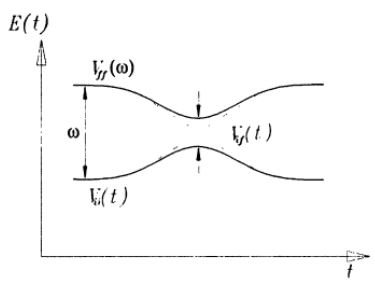
\includegraphics[width=70mm]{heavy_particle.JPG}}
	%\caption{\label{fig.2.4.1}}
\end{figure}



\subsection{Резонансная перезарядка}
\label{sec.2.5}

Резонансная перезарядка. Состоит в передаче электрона от одного ядра к другому в системе идентичных ядер: $A + A^{+} \rightarrow A^{+} + A$. Здесь, на первый взгляд, начальные и конечные состояния системы совпадают. Надо помнить, однако, что при этом происходит обмен скоростями между нейтральным атомом и ионом(направления движения каждого останется прежним)

Взаимодействие $V(R)$ в  определяющее переход электрона от одного ядра (атом) к другому (ион), определяется перекрытием волновых функций на двух ядрах, разделенных  
расстоянием $R$: $V(R)=exp(-\gamma R)$($\gamma=(2I)^{1/2}$ - определяется энергией связи $I$ электрона в атоме). Фактически при перезарядке электрон туннелирует между двумя потенциальными ямами.

\begin{figure}[h!]
	\center{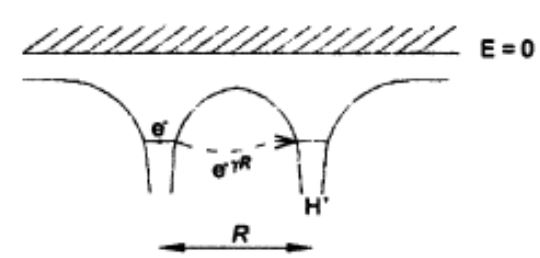
\includegraphics[width=70mm]{res_recharge.JPG}}
	%\caption{\label{fig.2.4.2}}
\end{figure}
 Вероятность перехода:
\begin{equation}
w(\rho)=sin^{2}[ \int_{-\inf}^{+inf} V(R(t))dt] \sim sin^{2}[V(\rho)\rho/v]
\end{equation}
Как следует из формулы, вероятность перехода между двумя ядрами быстро осциллирует при малых относительных скоростях v в соответствии с многократным перескоком электрона от одного ядра к другому, в результате чего электрон в среднем с вероятностью 1/2  находится в потенциальной яме каждого из ядер. Интегрируя свесом $2\pi\rho d\rho$, получим сечение резонансной перезарядки:
\begin{equation}
\sigma_{res}\propto(frac{pi}{2\gamma^{2}})ln^{2}(v_0/v)
\end{equation}

, где $v_0$ - скорость электрона на атомной орбите (порядка атомной). Видно, что сечение резонансной перезарядки значительно превышает атомные сечения благодаря большому значению логарифма  отношения атомной скорости к скорости относительного движения ядер.  Например, это сечение равно $5*10^{-15} см^{2}$ для перезарядки протона на водороде при энергии 1 эВ.

P.S. есть ещё и нерезонансная перезарядка при нерезонансной перезарядке, соответствующей передаче электрона от одного ядра к другому в случае неидентичных ядер с разными энергиями 
связи электрона на каждом из них.

Особый случай соответствует перезарядке атома на многозарядном ионе, потенциал ионизации которого намного превосходит потенциал ионизации исходного атома. Здесь атомный электрон переходит в густой спектр высоковозбужденных состояний многозарядного иона, для которых энергия связи близка к энергии связи в исходном атоме.
\begin{figure}[h!]
	\center{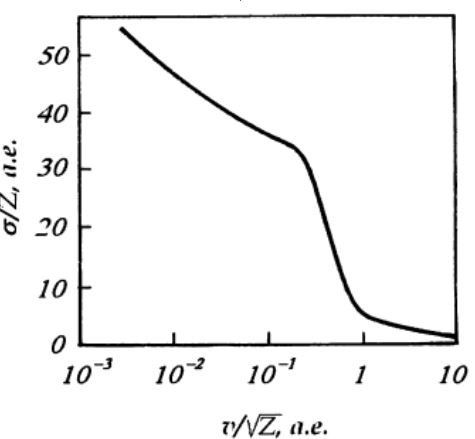
\includegraphics[width=70mm]{res_recharge_1.JPG}}
	%\caption{\label{fig.2.4.2}}
\end{figure}

Наверное, из всего надо вынести то, что при малых скоростях/энергиях налетающего атома, сечение будет большим, чтобы электрон за большое время пролёта стуннелировал в другой атом/ион. Экспериментально это и было подтверждено.(см рис.) В случае сильно искривлённого поля иона, туда ему стунелировать гораздо проще, поэтому сечение перезарядки $\sim Zn^{4}$, где z - заряд иона, n- номер орбиты

\subsection{Рекомбинация}
\label{sec.2.6}
Рекомбинация [Астапенко В.А.,Лисица В.С., столкновительные процессы в …... стр.99]


Трехчастичная рекомбинация является процессом, детально обратным процессу ионизации и, следовательно, записывается уравнением $A^{+Z} + 2e -> A^{+(Z-1)} + e $.Суть процесса трехчастичной рекомбинации состоит в том, что электрон плазмы, взаимодействующий с ионом, отдает избыток своей энергии другому электрону плазмы и захватывается на  уровень иона. Ясно, что рассматриваемый процесс может играть доминирующую роль в плазме с достаточно высокой плотностью (чтобы присутствие третьей частицы было вероятным) и низкой температурой (чтобы радиус кулоновского взаимодействия между частицами был велик). Оценим скорость рекомбинации:
\begin{equation}
\alpha_3 n^2_e N_i = k_{step} N_{neutr} n_e
\end{equation}

Подставляя из Саха-больцмана значение для соотношения $\frac{N_e N_i}{N_{neut}}$ получаем оценку для скорости ступенчатой ионизации
\begin{equation}
	k_{step}=\frac{C}{(2\pi)^{3/2}}\frac{g_i}{g_a}\frac{me^{10}}{\hbar^{3}T^{3}}exp(-I/T)
\end{equation}

Для сравнения этой скорости со скоростью прямой ионизации ($k_{dir}$)(как бы ионизация напрямую электроном с энергией равной энергии ионизации):
 \begin{equation}
 	k_{dir}=v_{el} \sigma_{dir}=\sqrt{2T/m} a_{0}^{2} exp(-I/T)
 \end{equation}

 \begin{equation}
 		\frac{k_{dir}}{k_{step}} \approx (\frac{T}{I})^{\frac{7}{2}}
 \end{equation}


Видно, что в плотной низкотемпературной плазме процессы ступенчатой (каскадной) ионизации преобладают над процессами прямой ионизации. 

Диэлектронная рекомбинация (ДР) является наряду с трехчастичной и радиационной одним из основных процессов образования ионов меньшей кратности в плазме с достаточно низкой плотностью, где преобладают процессы парных соударений. Для реализации этого вида рекомбинации необходимо наличие у рекомбинирующего иона некоторого числа остаточных электронов, т.е. электронного остова. Действительно, для одновременного выполнения законов сохранения энергии и импульса в процессе рекомбинации необходимо присутствие третьего тела, роль которого в случае трехчастичной рекомбинации играет электрон плазмы, а в случае радиационной (фото-) рекомбинации - световой квант. Точно так же при ДР роль третьего тела выполняет электронный остов иона, берущий на себя избыток энергии рекомбинирующего электрона.  ДР преобладает над трехчастичной рекомбинацией в достаточно разреженной плазме (малые ne) и при достаточно высокой температуре плазмы.

\subsection{Диссоциативная рекомбинация}
\label{sec.2.7}
\begin{figure}[h!]
	\center{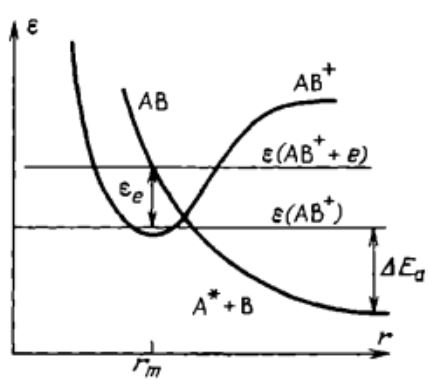
\includegraphics[width=70mm]{diss_recomb.JPG}}
	%\caption{\label{fig.2.4.2}}
\end{figure}
Первичным этапом диссоциативной рекомбинации является объединение молекулярного иона $АВ^{+}$ и электрона в квазимолекулу, которая находится в сверхвозбужденном автоионизационном состоянии. Соответствующая молекула $АВ$ может и не существовать, как в случае инертных газов, между атомами которых нет связи. Механизмом стабилизации захвата электрона ионом служит распад квазимолекулы на два атома; один из них может быть и возбужденным. Это возможно, если потенциальная кривая какого-либо из состояний системы атомов $А^{*} + В$ пересекает  потенциальную кривую иона $AB^{+}$. 
Системы $AB^{+} + e$ и $A^{*}+B$ при междуядерном расстоянии около $r_m$ имеют одинаковые энергии. Поэтому возможен самопроизвольный переход из первой конфигурации во вторую. 
Коэфициент диссоциативной рекомбинации равен:
\begin{equation}
\beta_{dis}=k_{capt}\frac{w_{stab}}{w_{stab}+w_{auto}}=\frac{k_{capt}}{w_{auto}}\frac{w_{stab}w_{auto}}{w_{stab}+w_{auto}}
\end{equation}
, где  $w_{auto} [c^{-1}]$- вероятность стабилизации (как и с излучением фотона - по факту обратное время жизни состояния) $w_{stab}\sim v_a[см/с] / a[см]$ скорость и размер частиц соответственно. Получается $w_{stab} \approx 10^{14} c^{-1}$, то есть это оч быстрый процесс. Он происходит даже быстрее, чем высвечивание кванта ($10^{8} c^{-1}$ )


\subsection{Прилипание.}
\label{sec.2.8}

 [райзер, стр. 145]
 
 
Процессы прилипания (attachment), сопровождающиеся образованием отрицательных ионов, важны для разрядов по двум причинам. Когда в тех газах, которые используются для исследований или приложений, имеются электроотрицательные компоненты, прилипание может играть заметную, иногда даже главную роль среди механизмов потерь электронов.
Они не зависят от механизмов образования и разрушения ионов и определяются уравнением Саха, в котором по смыслу роль положительных ионов играют нейтральные частицы, а роль атомов и молекул — отрицательные ионы:
\begin{equation}
	\frac{n_{-}}{n_e}=N\frac{g_{-}}{g_{a}}\frac{e^{I_{-}/kT}}{AT^{3/2}}
\end{equation}



\section{Колебания и волны в плазме}
\label{sec.7}

\subsection{Столкновения заряженных частиц, дальнодействие.}
\label{sec.2.1}
В изотропной плазме легко записат дисперсионное уравнение:

\begin{equation}
    \label{eq.Disp1}
    \left(1-\frac{\omega^2}{c^2 k^2} \varepsilon_{\perp}\right) E_{\perp} + \varepsilon_{\parallel} * E_{\parallel}= 0
\end{equation}

Отсюда, при условии $\varepsilon_{\parallel} = 0$ получаем первый тип волн - продольные(ленгмюровские/электростатические) 
волны. Затухание Ландау(безстолкновительное затухание) относится именно к таким волнам. Их дисперсионка имеет следующий
вид:

\begin{equation}
    \label{eq.Disp2}
    \omega=\omega_p + 3/2 (k v_{t})^2
\end{equation}
волны с частотой сильно отличной от плазменное затухают(т.е. это плазменное колебание).

В случае $1 - \frac{\omega^2}{c^2 k^2} \varepsilon_{\parallel}=0$ получаем поперечные волны(почти как в вакууме). Для них
дисперсионка:

\begin{equation}
    \label{eq.Disp3}
    \omega^2=\omega_p^2 + (c k)^2
\end{equation}
Легко видеть, что волны с частотой $\omega < \omega_p$ не распространяются.

Если еще учесть ионы:

\begin{equation}
    \label{eq.Disp4}
    \varepsilon=1+\frac{\omega_{pe}^2}{k^2 v_{Te}^2} - \frac{\omega_{pi}^2}{\omega^2}-3\frac{\omega_{pi}^2 k^2 v_{Ti}^2}{\omega^4}
\end{equation}
В случае низких частот(где влияние ионов существенно) можно принебреч 4ым слашаемым, тогда дисперсионка примет следующий вид:

\begin{equation}
    \label{eq.Disp5}
    \omega=\frac{k c_s}{\sqrt{1 + k^2 r_d^2}}
\end{equation}
при малых $k$ имеем $\omega=k c_s$, где $c_s=\frac{T_i + T_e}{M}$ (ионный звук).

Магнитоактивная плазма
Рассмотрим сначала магнито-звуковые волны. 
При наличии внешнего магнитного поля $B_0$. Будем рассматривать холодную плазму. Вводя обозначения $n^2=\frac{c^2 k^2}{\omega^2}$, $\upsilon=\frac{\omega_p^2}{\omega^2}$, $u=\frac{\omega_H^2}{\omega^2}$, где $\omega_H$ - циклотронная частота
дисперсионку можно записать следующим образом:

\begin{equation}
    \label{eq.Disp5}
    n_{e,o}^2=1-\frac{2\upsilon (1-\upsilon)}{2(1-\upsilon) - u \sin^2(\theta) \pm \sqrt{u^2 \sin^4(\theta) + 4u(1-\upsilon)^2 \cos^2(\theta)}} 
\end{equation}
где $\theta$ это угол между магнитным полем и волновым вектором. Индексы e,o соответствуют необыкновенной и обыкновенной волнам.




\section{Прикладные проблемы физики плазмы}
\label{sec.14}



\subsection{Управляемый термоядерный синтез}
\label{14}

[Кенро Миямото, Основы Физики Плазмы и управляемого термоядерного синтеза, Москва, физматлит 2007]

Всем известно про дефект масс, что при слиянии ядер до Fe и Ni выделяется энергия.
основная реакция D+T-> 4He + n [17.59 MeV], 1/5 энергии приходится на He и 4/5 на n
Чтобы сблизить ядра на достаточное расстояние надо преодолеть кулоновский барьер. ту силу, с которой они отталкиваются ($Z_{alpha}Z_p e^2/r_N$) вычислили, что примерное расстояние $r_{n}=1.4*10^{-13}*(A^{1/3}_{\alpha}+A^{1/3}_{\beta}) [cm]$ Но это оказалось слишком мало, ибо не сходилось с вычислениями T солнца, для 10кэВ вычислили точку остановки $R_t=10^{-11} [cm]$

[Миямото стр. 23]

Почему вообще надо удерживать плазму, какие характерные времена? Критерий Лоунсена 
Дело обстоит в том, что система должна сама себя поддерживать и при этом отдавать эл. энергию. Энергия в единице объёма $(3/2)nk(T_i+T_e)$. Время остывания $\tau_E = \frac { (3/2)nk(T_i+T_e) }{P_L+R}$, , где $P_L$ и $R$ соответственно мощность потерь энергии на диффузию и излучение плазмой. В то же время, в объёме происходит выделение тепла за счёт термоядерного синтеза мощностью. $P_{NF}=(n/2)(n/2)<\sigma v> Q_{NF} $. Потому
 как D и T присутствуют в реакторе в равном количестве и концентрация каждого n/2 соответственно. $<\sigma v> $ - вероятность процесса,   $Q_{NF} $ энергия на одну реакцию.
Чтобы всё было устойчиво и не затухало: $P_{heat}=P_L + R = \frac{3nkT}{\tau_E} < \eta_{el} \eta_{heat} P_{NF} $, где $\eta_{el} $ - КПД получения эл. мощности ,$ \eta_{heat} $ - КПД нагрева.

Итого: $ \frac{3nkT}{\tau_E} < \eta_{el} \eta_{heat} Q_{NF} n^{2} \frac{<\sigma v>}{4}$

\begin{equation}
	\label{eq.Disp14.1.1}
	n \tau_E > \frac{12 kT}{\eta Q_{NF} <\sigma v>} > 1.7*10^{20} m^{-3} s
\end{equation}
 - Критерий Лоунсена , критерий термоядерности. То есть надо или увеличивать концентрацию, или время удержания. Поэтому есть как токамаки с непрерывным временем работы, так и импульсные(импульсно поддерживается магнитное поле).
Понятно, что чем горячее плазма, тем труднее её удерживать, понятно что удерживать надо именно магнитным полем.

\subsection{Магнитное удержание}
\label{14.1}

Уравнения магнитной гидродинамики тут написаны [Голант Жилинский Сахаров, Основы ФП,  §10.1]

Из уравнения для средней скорости $\rho (du/dt)=(1/c)[j H]-grad\;p$; где $p=p_e+p_i$ - суммарное давление, $j=en(u_i+u_e)$ - плотность тока, $ du/dt=\delta u / \delta t + (u grad)u$ полная производная

можно вывести условие равновесия
\begin{equation}
	\label{eq.Disp14.1.2}
	\frac{1}{c}[j H]=grad\;p
\end{equation}
[Голант Жилинский Сахаров, Основы ФП,  §10.2]


Идея состоит в том, что преодолеть давление плазмы как газа с ооочень большой температурой с помощью давления магнитного поля около стенок.
Первая задача, возникающая при рассмотрении удержания плазмы в магнитном поле, заключается в определении условий, при которых достигается равновесие, т. е. электродинамические силы, действующие на каждый элемент объема плазмы, уравновешивают градиент давления.
\begin{equation}
	\label{eq.Disp14.1.3}
	G_H=\frac{1}{c} [j H]=\frac{1}{4 \pi} [H rotH]=-\frac{1}{8 \pi} grad(H^{2})+\frac{1}{4 \pi} (H grad) H
\end{equation}
Так же есть отдельный случай, когда линии имеют радиус кривизны R.

\begin{equation}
	\label{eq.Disp14.1.4}
(\vec H grad)\vec H=H(\vec h grad)\vec h H=H^{2} grad_{||}\vec h + \frac{1}{2} grad_{||} H^{2}=-H^{2} \frac{\vec R}{R}+\frac{1}{2} grad_{||} H^{2}
\end{equation}


, где $\vec h= \frac{\vec H}{H}$; $grad_{||}=(\vec h \; grad)$ - проекция градиента на направление магнитного поля. Подставляем в предыдущее выражение и получаем, что давление:
\begin{equation}
	\label{eq.Disp14.1.5}
 G_H=-grad_{\perp}(H^{2}/8\pi)-(H^{2}/4\pi R^{2})\vec R
\end{equation}
Первое слагаемое в представляет собой поперечный градиент введённого магнитного давления. Действие этой силы можно описать как взаимное «расталкивание» силовых линий в поперечном направлении. Второе слагаемое определяет силу, направленную к центру кривизны силовых линий, и называется натяжением магнитного поля. Оно формально получается, если приписать силовым линиям свойства растянутой струны.

Для равновесия: 
\begin{equation}
	\label{eq.Disp14.1.6}
 grad p + grad_{\perp}(H^{2}/8\pi)+(H^{2}/4\pi R^{2})\vec R =0
\end{equation}

Для случая, когда силовые линии прямые ($R\rightarrow \inf $), уравнение сводится к постоянству суммы кинетического и магнитного давлений в плоскости, перпендикулярной магнитному полю:
\begin{equation}
	\label{eq.Disp14.1.7}
p + H^{2}/8\pi=const
\end{equation}
\begin{equation}
	\label{eq.Disp14.1.8}
p_0 + H_{0}^{2}/8\pi=H_{e}^{2}/8\pi
\end{equation}

Равенство показывает, что максимальное давление плазмы, которое можно удерживать магнитным полем, равно магнитному давлению вне плазмы $H_{e}^{2}/8\pi$. При описании магнитного удержания часто вводят коэффициент $\beta$, представляющий собой
отношение давления удерживаемой плазмы к максимально возможному: $\beta=p/p_{max}=8\pi p/H_{e}^{2}$
Но это удержание поперёк линий магнитного поля, а строить комплексы в виде торов не всегда удобно, поэтому было придумано пробочное удержание.

пробочное удержание [Миямото стр. 32]

Понятно, что всё движение электрона в магнитном поле можно описать как движение вдоль и поперёк поля. Вдоль - свободное движение, поперёк - ларморовское вращение.
Если рассмотрим электрон в поле, он будет вращаться по кругу с радиусом равному Ларморовскому. Его можно представить в виде витка с током. У витка с током есть магнитный момент.
\begin{equation}
	\label{eq.Disp14.1.9}
 \mu=I*S=\frac{q\Omega}{2\pi} * \pi \frac{\rho^{2}}{2}=\frac{mv_{perp}^{2}}{2B}
\end{equation}	
Но кин энергия должна сохранятся при движении в магнитном поле, поэтому электрон будет лететь вдоль поля пока
\begin{equation}
	\label{eq.Disp14.1.10}
	\frac{mv_{||}^{2}}{2}+\frac{mv_{\perp}^{2}}{2}=\frac{mv^{2}}{2}=const
\end{equation}	
Поскольку магнитный момент сохраняется, то:
\begin{equation}
	\label{eq.Disp14.1.11}
 v_{||}=+-(\frac{2}{m}E-v_{\perp}^{2})^{1/2}=+-(v^{2}-\frac{2}{m} \mu B)^{1/2}
\end{equation}	
То есть электрон может полностью убрать продольную скорость и отразиться. Почему возникает этот эффект ? Потому что на магнитный диполь действует сила $-\mu \grad_{||}$ B. Ну и вводится пробочное отношение - отношение магнитных полей в центре и на краях ловушки $R_M=\frac{B_M}{B_0}$

\newpage
\addcontentsline{toc}{section}{Список литературы}
\bibliographystyle{unsrt}
\bibliography{program}

\end{document}